\documentclass[11pt,a4paper,bibliography=totoc,abstract=true]{scrartcl}

% --- SPRACHE UND SCHRIFTARTEN ---
\usepackage[ngerman]{babel}
\usepackage[T1]{fontenc}
\usepackage[utf8]{inputenc}
\usepackage{mathptmx} % Times-compatible font for main text
\usepackage[scaled=0.92]{helvet} % Arial-compatible sans-serif
\usepackage{microtype}
\usepackage{geometry}
\usepackage{setspace}
\usepackage{amsmath,amssymb}
\usepackage{graphicx}
\usepackage{booktabs}
\usepackage{tabularx}
\usepackage{array}
\usepackage{siunitx}
\usepackage{eurosym}
\usepackage{caption}
\usepackage{subcaption}
\usepackage{float}
\usepackage{xcolor}
\usepackage{tikz}
\usepackage{pgfplots}
\usepackage{csquotes}
\usepackage{xspace} % Verhindert das Verschlucken von Leerzeichen nach Makros
\usepackage{listings} % Benötigt für Code-Anzeigen
\usepackage{hyperref}
\usepackage[nameinlink,noabbrev]{cleveref}
\usepackage[backend=biber,style=authoryear,sorting=nyt]{biblatex}
% Anmerkung zum Zitationsstil: Im Fachbereich Computer Vision / Machine Learning ist das
% Autor-Jahr-System (APA/Chicago-Style) etablierter Standard. Die vorliegende Arbeit folgt
% dieser Konvention, um die Nachvollziehbarkeit innerhalb der internationalen Forschungsgemeinschaft
% zu gewährleisten. Webquellen enthalten gemäß Leitfaden-Anforderung vollständige URL und Zugriffsdatum.

% Format citations to match Leitfaden: Author, Year
\DeclareCiteCommand{\cite}[\mkbibparens]
  {\usebibmacro{prenote}}
  {\usebibmacro{citeindex}%
   \printtext[bibhyperref]{\usebibmacro{cite}}}
  {\multicitedelim}
  {\usebibmacro{postnote}}

\DeclareCiteCommand{\autocite}[\mkbibparens]
  {\usebibmacro{prenote}}
  {\usebibmacro{citeindex}%
   \printtext[bibhyperref]{\usebibmacro{cite}}}
  {\multicitedelim}
  {\usebibmacro{postnote}}

\renewcommand*{\nameyeardelim}{\addcomma\space}

% Der Leitfaden fordert mindestens 10 pt. Bei 11 pt Grundschrift bleiben auch
% Beschriftungen und Fußnoten in der Regel mindestens 10 pt groß.
\captionsetup{font=normalsize}
\renewcommand{\footnotesize}{\fontsize{10}{12}\selectfont}

% --- CODING STYLE DEFINITION (Verhindert den Compiler-Absturz!) ---
\definecolor{codegreen}{rgb}{0,0.6,0}
\definecolor{codegray}{rgb}{0.5,0.5,0.5}
\definecolor{codepurple}{rgb}{0.58,0,0.82}
\definecolor{backcolour}{rgb}{0.95,0.95,0.92}

\lstdefinestyle{pythonstyle}{
    backgroundcolor=\color{backcolour},   
    commentstyle=\color{codegreen},
    keywordstyle=\color{blue},
    numberstyle=\footnotesize\color{codegray},
    stringstyle=\color{codepurple},
    basicstyle=\ttfamily\footnotesize,
    breakatwhitespace=false,         
    breaklines=true,                 
    captionpos=b,                    
    keepspaces=true,                 
    numbers=left,                    
    numbersep=5pt,                  
    showspaces=false,                
    showstringspaces=false,
    showtabs=false,                  
    tabsize=4,
    inputencoding=utf8,
    extendedchars=true,
    literate={ä}{{\"a}}1 {ö}{{\"o}}1 {ü}{{\"u}}1 {Ä}{{\"A}}1 {Ö}{{\"O}}1 {Ü}{{\"U}}1 {ß}{{\ss}}1
}

% --- FORM NACH JUGEND-FORSCHT-LEITFADEN (Stand Juli 2025) ---
\geometry{left=2.5cm,right=2.5cm,top=2.5cm,bottom=2.5cm}
\onehalfspacing
\setlength{\parindent}{0pt}
\setlength{\parskip}{0.45em}
\setcounter{secnumdepth}{3}
\setcounter{tocdepth}{2} % Zeigt Abschnitte (1) und Unterpunkte (1.1) an
\pgfplotsset{compat=1.18}
\sisetup{detect-all}

% --- HYPERREF SETUP (Klickbare blaue Links mit Hover-Effekt) [2] ---
\hypersetup{
  colorlinks=true,                  % Aktiviert farbigen Text für Links [2]
  linkcolor=blue!75!black,          % Interne Links (Inhaltsverzeichnis, Referenzen) werden blau [2]
  citecolor=green!50!black,         % Zitate werden grün
  urlcolor=blue!70!black,           % Weblinks werden blau
  pdftitle={MIRA - Machine Intelligence for Recycling Automation},
  pdfauthor={Jeremy Darko}
}

\graphicspath{{figures/}}

\addbibresource{references.bib}

% Makro mit xspace-Unterstützung für fehlerfreien Fließtext
\newcommand{\mira}{\textsc{MIRA}\xspace}

\begin{document}

% ==============================================================================
% NICHT MITGEZÄHLT: Deckblatt, Projektüberblick und Inhaltsverzeichnis
% ==============================================================================
\pagenumbering{roman} % Römische Seitenzahlen für den Vorspann [2]

% 1. Titelseite
\begin{titlepage}
    \centering
    \vspace*{1.5cm}
    {\large\textbf{JUGEND FORSCHT 2027}\par}
    \vspace{0.35cm}
    {\large Regionalwettbewerb Nordrhein-Westfalen (Ruhrgebiet)\par}
    {\large Fachgebiet: Technik\par}

    \vspace{2.2cm}
    {\huge\bfseries MIRA\par}
    \vspace{0.45cm}
    {\Large\bfseries Machine Intelligence for Recycling Automation\\}
    {\large Edge-KI-basierte Erkennung und mechatronische Sortierung von Sekundärrohstoffen\par}

    \vspace{2.3cm}
    \begin{tabular}{ll}
        \textbf{Jungforscher:} & Jeremy Darko \\
        \textbf{Jahrgangsstufe:} & Stufe EF (Jahrgangsstufe 11) \\
        \textbf{Schule:} & Gymnasium Broich \\
        \textbf{Schulort:} & Mülheim an der Ruhr \\
        \textbf{Datum der Einreichung:} & 15. Januar 2027 \\
    \end{tabular}

    \vfill
    {\small Projekt-Repository: \url{https://github.com/jeremy341/MIRA-AI}\par}
\end{titlepage}

% 2. Projektüberblick (maximal eine Seite)
\clearpage
\section*{Projektüberblick}
\addcontentsline{toc}{section}{Projektüberblick}

MIRA ist ein Softwareprototyp, der Glas, Metall, Papier, Kunststoff und Restmüll in Kamerabildern erkennen und lokalisieren soll. Untersucht wird, welcher messbare Zielkonflikt zwischen Erkennungsqualität, Modellgröße und CPU-Latenz entsteht, wenn ein kompaktes Detektionsmodell trainiert und auf INT8 quantisiert wird. Ein erster, abgeschlossener Machbarkeitsnachweis (Stage~A) verglich Bildklassifikatoren für vier Wertstoffklassen. Historische Detektionsläufe EXP-013 bis EXP-017 verwendeten anschließend YOLO11n und unterschiedliche Mischungen öffentlicher Datensätze; ihre Ergebnisse dienen als Ausgangspunkt, stammen aber nicht aus dem neu aufgebauten Datensatz. Dieser aktuelle, annähernd nach Objektannotationen ausgeglichene Fünfklassen-Datensatz umfasst getrennte Trainings-, Validierungs- und Testsätze. Der zugehörige Trainings- und Quantisierungsvergleich steht noch aus. Ein Raspberry Pi, eine Kamera und ein Sortierarm sind als spätere Integrationsstufe geplant und wurden in der vorliegenden Softwareuntersuchung noch nicht vermessen.

\clearpage

% 3. Inhaltsverzeichnis
\tableofcontents
\clearpage

% ==============================================================================
% MITGEZÄHLT: Fachliche Kurzfassung bis einschließlich Fazit und Ausblick
% ==============================================================================
\pagenumbering{arabic}
\setcounter{page}{1}

\section*{Fachliche Kurzfassung}
\addcontentsline{toc}{section}{Fachliche Kurzfassung}

Die vorliegende Arbeit evaluiert systematisch mehrere Deep-Learning-Architekturen für die automatische Klassifikation und Detektion von Recyclingmaterialien auf ressourcenbeschränkter Edge-Hardware \autocite{yosinski2014transferable}.
Ein Vergleich eines Scratch-CNNs, eines vortrainierten MobileNetV2 mit Transfer Learning sowie eines YOLO11n-Modells zeigt, dass Post-Training-Quantisierung (INT8) die Modellgröße des fine-tuned MobileNetV2 um einen Faktor 9 auf \SI{2.61}{\mega\byte} komprimiert, bei einem vernachlässigbaren Genauigkeitsverlust von 0,07 Prozentpunkten \autocite{krishnamoorthi2018quantizing,deng2020model}.
Das fine-tuned MobileNetV2 erreicht eine Validierungsgenauigkeit von \SI{87.42}{\percent} und übertraf das Scratch-CNN um \num{26.42} Prozentpunkte; YOLO11n erzielt auf der besten Datensatzkombination \SI{60.7}{\percent} mAP50 \autocite{ultralyticsyolov8,proenca2020taco,yang2016classification}.
Die Ergebnisse deuten auf die Machbarkeit echtzeitfähiger, kostengünstiger Sortiersysteme hin, die auf ressourcenbeschränkter Edge-Hardware (Raspberry Pi Zero 2W oder Raspberry Pi 4) betrieben werden können.

\clearpage
\section{Einleitung und Motivation}

\subsection{Problemstellung}
Getrennt erfasste Abfälle können nur dann gezielt weiterverarbeitet werden, wenn Materialarten zuverlässig unterschieden werden. Kamerabasierte Objekterkennung ist dafür ein möglicher Baustein: Sie liefert zu einer Klasse auch die Position eines Gegenstands im Bild. Visuell ähnliche oder verformte Gegenstände, wechselnde Hintergründe und begrenzte Rechenleistung erschweren jedoch den Einsatz. MIRA untersucht dieses Problem zunächst als reproduzierbaren Softwareprototyp; Aussagen über die Sortierleistung einer vollständigen Anlage sind damit noch nicht möglich.

\subsection{Ziel und Forschungsfrage}
Ziel ist eine nachvollziehbare Pipeline für fünf Klassen: \textit{glass, metal, paper, plastic} und \textit{trash}. Im Mittelpunkt steht nicht der Nachweis eines fertigen Sortierroboters, sondern die folgende Forschungsfrage:

\begin{quote}
\emph{Welcher messbare Zielkonflikt zwischen Detektionsgüte, Modellgröße und CPU-Latenz ergibt sich beim Training und bei der INT8-Quantisierung eines kompakten YOLO11n-Modells für fünf Abfallklassen?}
\end{quote}

Die Detektionsgüte wird mit mAP50--95 als Hauptmetrik sowie mAP50, Precision, Recall und dem schwellenwertabhängigen $F_1$-Score beschrieben. Modellgröße und Latenz werden für dasselbe exportierte Modell erfasst. Messungen auf einem Raspberry Pi und die Kopplung an einen Roboterarm bilden eine spätere Projektstufe.

\subsection{Themenfindung}
Die Projektidee entstand aus Beobachtungen der Mülltrennung im schulischen Alltag und bei Besuchen lokaler Recyclinghöfe. Daraus entwickelte sich die technische Frage, wie weit eine kleine, lokal ausführbare Computer-Vision-Pipeline mit dokumentierten Daten und Messgrößen kommt.

\subsection{Abgrenzung der Projektphasen}
Stage~A ist ein abgeschlossener Machbarkeitsnachweis zur Klassifikation einzelner Bilder in vier Klassen. Die späteren EXP-013 bis EXP-017 sind historische Fünfklassen-Detektionsläufe mit unterschiedlichen Datenmischungen. Sie motivieren die aktuelle Untersuchung, ersetzen wegen ihrer unterschiedlichen Datengrundlagen aber keinen kontrollierten Vergleich. Der neu aufgebaute, annähernd ausgeglichene Datensatz und der darauf geplante Lauf bilden den aktuellen Arbeitsstand. Raspberry Pi, Kameraaufbau und Roboterarm sind noch nicht experimentell integriert.

\subsection{Aufbau der Arbeit}
Nach den notwendigen Grundlagen werden Datensätze, Trennregeln und Messgrößen beschrieben. Anschließend folgen Implementierung, bisherige Ergebnisse, deren Grenzen und die geplanten nächsten Versuche.

\section{Theoretische Grundlagen}

\subsection{Edge AI und Ressourceneffizienz}
Die herkömmliche Verarbeitung von Machine-Learning-Modellen erfolgt meist auf leistungsstarken Cloud-Servern mit dedizierter Grafikbeschleunigung (GPU). Im Kontext der dezentralen Wertstoffsortierung stößt dieser Ansatz jedoch auf signifikante Hürden: Hohe Latenzzeiten bei der Datenübertragung, Abhängigkeit von einer permanenten Internetverbindung und erhebliche Betriebskosten. 

Das Paradigma der \emph{Edge AI} beschreibt die Ausführung von KI-Modellen direkt auf lokalen, ressourcenbeschränkten Endgeräten wie Einplatinencomputern (z.B. Raspberry Pi) oder Mikrocontrollern \cite{deng2020model, wang2020survey}. Für ein mechanisches Sortiersystem wie \mira ergeben sich daraus drei kritische Zielgrößen, die in einem permanenten Spannungsverhältnis stehen:
\begin{enumerate}
    \item \textbf{Minimierung der Modellgröße:} Der lokale Speicher (RAM/Flash) ist stark begrenzt \cite{deng2020model}.
    \item \textbf{Maximierung der Inferenzgeschwindigkeit:} Um Objekte auf einem bewegten Förderband präzise zu greifen, muss die Latenz im zweistelligen Millisekundenbereich liegen \cite{deng2020model}.
    \item \textbf{Erhaltung der Robustheit:} Das System muss trotz wechselnder Beleuchtung und verrauschter Hintergründe stabile Vorhersagen liefern.
\end{enumerate}

Die technologische Herausforderung besteht darin, diese drei Parameter durch gezielte Modellwahl und Kompressionstechniken zu optimieren \cite{deng2020model}.

\subsection{Convolutional Neural Networks (CNNs)}
Für Aufgaben der Computer Vision haben sich Convolutional Neural Networks (CNNs) als Standard etabliert \cite{lecun2015deep, bengio2013representation}. Im Gegensatz zu klassischen, vollverknüpften Netzen nutzen CNNs die räumliche Struktur von Bildern aus, indem sie Merkmale schrittweise über zweidimensionale Faltungsoperationen extrahieren. Frühe Schichten lernen elementare geometrische Strukturen wie Kanten und Farbgradienten, während tiefere Schichten diese zu komplexen semantischen Konzepten kombinieren. Nachgeschaltete Aktivierungsfunktionen wie die Rectified Linear Unit ($\text{ReLU}(x) = \max(0, x)$) führen Nichtlinearitäten ein, und eine abschließende Softmax-Schicht wandelt die berechneten Rohwerte in eine Wahrscheinlichkeitsverteilung über die Klassen um.

Die Evaluierung der Modellgüte erfolgt über Precision / Recall und den $F_1$-Score:
\begin{equation}
F_1 = 2 \cdot \frac{\text{Precision} \cdot \text{Recall}}{\text{Precision} + \text{Recall}}
\end{equation}

\subsection{Transfer Learning und MobileNetV2}
Das Training tiefer Netze von Grund auf erfordert zehntausende annotierte Bilder. Beim \emph{Transfer Learning} wird ein auf einem sehr großen Datensatz (ImageNet mit 1,4 Millionen Bildern) vortrainiertes Modell als Feature-Extractor wiederverwendet \cite{yosinski2014transferable}. 

Als Rückgrat (Backbone) der Klassifikationsstufe von \mira wurde die MobileNetV2-Architektur gewählt \cite{sandler2018mobilenetv2}. Diese ist speziell für mobile Endgeräte optimiert und basiert auf \emph{Depthwise Separable Convolutions}. Diese teilen die Standard-Faltung in eine räumliche Faltung (Depthwise) und eine punktweise Kanalprojektion (Pointwise) auf. Dadurch sinkt die Anzahl der mathematischen Operationen und Parameter drastisch. Eine Standard-Faltung mit Kernelgröße $k \times k$, $C_{\text{in}}$ Eingabekanälen und $C_{\text{out}}$ Ausgabekanälen erfordert $k \times k \times C_{\text{in}} \times C_{\text{out}}$ Multiplikationen pro Pixel. Die depthwise-separable Variante zerlegt dies in einen räumlichen Filter ($k \times k \times C_{\text{in}}$) und eine punktweise $1 \times 1$-Kanalprojektion ($C_{\text{in}} \times C_{\text{out}}$), wodurch die Rechenkomplexität um einen Faktor von ungefähr $k^2$ (bei typischen $3 \times 3$-Kerneln ca.\ $8$--$9 \times$) reduziert wird. Diese Dekomposition ist möglich, da räumliche und kanalbezogene Korrelationen in Bildern weitgehend entkoppelt vorliegen. 

MobileNetV2 nutzt zudem \emph{Inverted Residual Blocks} mit \emph{Linear Bottlenecks}, um den Informationsverlust in schmalen Schichten zu minimieren. Die „invertierte" Struktur erweitert die Kanaldimension zunächst (Expansionsfaktor $6 \times$), wendet die Depthwise-Faltung an und komprimiert anschließend wieder zurück -- im Gegensatz zum klassischen ResNet-Bottleneck, der zuerst komprimiert. Die lineare (ReLU-freie) Bottleneck-Schicht verhindert Informationsverlust in der niedrigdimensionalen Projektion, und Skip-Connections überspringen die dünne Bottleneck-Schicht direkt. Im Projekt wurde der Backbone zunächst eingefroren, um generische Filter zu erhalten, und anschließend ab Layer 100 feingetunt, um sich an die spezifischen Reflexionen von Wertstoffen anzupassen. Die Fein-Tuning-Parameter umfassen den Adam-Optimierer mit Lernrate $\eta = 10^{-5}$, 15 Trainingsepochen und eine Batch-Größe von 32. Die ersten 100 Schichten des MobileNetV2-Backbones bleiben eingefroren; ab Schicht 100 werden insgesamt 1.866.564 Parameter feingetunt (von 2.263.108 gesamt).

\subsection{Post-Training-Quantisierung (INT8)}
Die Post-Training-Quantisierung (PTQ) reduziert Modellgröße und Rechenaufwand durch Umwandlung in INT8-Formate. Die Quantisierungsabbildung lautet kompakt
\begin{equation}
q = \mathrm{round}\left(\frac{r}{S}\right) + Z
\end{equation}
mit kontinuierlichem Wert $r$, Skalierungsfaktor $S$ und Nullpunkt $Z$.

Die Reduktion von FP32 auf INT8 funktioniert, weil die Gewichte und Aktivierungen eines neuralen Netzwerks typischerweise in einem engen Wertebereich konzentriert sind \cite{krishnamoorthi2018quantizing}. Ganzzahlarithmetik (INT8) ist auf ARM-Prozessoren mit NEON-SIMD-Einheit deutlich effizienter als Gleitkommaarithmetik (FP32), da die Integer-Alu höhere Durchsatzraten bei niedrigerer Leistungsaufnahme erreicht. Für MIRA wurde eine Kalibrierung mit 100 repräsentativen Trainingsbildern durchgeführt, deren Aktivierungsbereiche (min/max) die Skalierungsfaktoren $S$ und $Z$ bestimmen \cite{krishnamoorthi2018quantizing}. Ein potenzielles Risiko stellt die Sättigung (Clipping) dar: Werden Ausreißer-Aktivierungen abgeschnitten, kann dies zu systematischen Fehlern führen, weshalb die Kalibrierungsstichprobe repräsentativ sein muss.

\subsection{Echtzeit-Objekterkennung mit You Only Look Once (YOLO11n)}
Für den mechatronischen Sortierprozess reicht eine reine Klassifikation ("Was ist im Bild?") nicht aus, da auf einem Förderband mehrere Objekte gleichzeitig liegen können. Das System benötigt exakte Ortskoordinaten.

MIRA nutzt hierfür das Single-Shot-Detektionsmodell YOLO11n \cite{ultralyticsyolov8}. YOLO-Architekturen \cite{redmon2016yolo} verzichten auf komplexe, zweistufige Vorschlagsnetzwerke wie Faster R-CNN \cite{ren2015faster} und berechnen stattdessen in einem einzigen Vorwärtspass (Single Pass) über ein neuronales Netz sowohl die Begrenzungsrahmen (Bounding Boxes) als auch die Klassenwahrscheinlichkeiten für jedes Objekt. Konkret unterteilt YOLO das Eingabebild in ein $S \times S$ Raster; jede Rasterzelle sagt Begrenzungsrahmen, einen Objektscore (Klassenwahrscheinlichkeit $\times$ Überlappungsgrad) und Klassenwahrscheinlichkeiten vorher. Nicht-maximale Unterdrückung (Non-Maximum Suppression, NMS) \cite{neubeck2006efficient} eliminiert dabei überlappende Vorhersagen desselben Objekts.

In den frühen Experimenten (EXP-005 bis EXP-008) wurde YOLOv8-Nano als Ausgangsarchitektur verwendet. Ab EXP-013 wurde auf YOLO11n migriert, dessen aktualisierte Architektur eine effizientere Feature-Pyramide und verbesserte Loss-Funktionen bietet.

\subsection{Temporale Signalstabilisierung (EMA-Filter)}
In der Live-Inferenz wurde ein EMA-Filter zur Dämpfung von Fluktuationen verwendet:
\begin{equation}
p_{\mathrm{smooth}}(t)=\alpha\,p_{\mathrm{raw}}(t)+(1-\alpha)\,p_{\mathrm{smooth}}(t-1)
\end{equation}
Im Projekt wurde $\alpha=0{,}15$ gewählt (siehe Anhang für Parameterstudie).
\section{Methodik und Experimentdesign}

\subsection{Stage A: abgeschlossener Klassifikationsvorversuch}
Stage~A verwendete 796 unter kontrollierten Bedingungen aufgenommene Bilder der Klassen \textit{glass, metal, paper} und \textit{plastic}. Mit Seed~123 wurden \SI{80}{\percent} für Training und \SI{20}{\percent} für Validierung vorgesehen (etwa 637/159 Bilder). Verglichen wurden ein kleines CNN, MobileNetV2 mit eingefrorenem Backbone, Fine-Tuning und der INT8-Export \cite{sandler2018mobilenetv2,tensorflow2024transfer}. Eingabegrößen und Vorverarbeitung waren innerhalb des jeweiligen Modellvergleichs festgelegt. Stage~A bewertet Bildklassifikation mit Accuracy; ihre Resultate sind nicht mit mAP-Werten der Detektion gleichzusetzen.

\subsection{Historische Detektionsentwicklung}
\label{sec:method-gigo}
Für die Objekterkennung werden Bounding Boxes benötigt. Ein früher Auto-Labeling-Versuch mit Canny-Kanten und Otsu-Schwellenwert erfasste häufig kontrastreiche Tischbereiche statt der Gegenstände. Das zugehörige EXP-005 war deshalb kein belastbarer Nachweis der Generalisierung. Danach wurden unter anderem TACO, Roboflow Trash Detection und ein mithilfe von SAM nachannotierter TrashNet-Bestand eingesetzt \cite{proenca2020taco,roboflow2023trash,yang2016classification,kirillov2023segment}.

Die YOLO11n-Läufe EXP-013 bis EXP-017 sind historische Experimente. EXP-013 nutzte TACO und TrashNet, EXP-014 zusätzlich Roboflow, EXP-015 TACO, TrashNet und WaRP, EXP-016 nur WaRP und EXP-017 alle vier Quellen \cite{warp2024dataset,ultralyticsyolov8}. Sie liefen jeweils 120 Epochen mit $640\times640$ Pixeln. Da sich Zusammensetzung und resultierende Validierungsbestände änderten, werden ihre mAP-Werte deskriptiv berichtet, aber nicht als kontrollierte Ablation oder als Resultat des aktuellen Datensatzes interpretiert.

\subsection{Aktueller balancierter Fünfklassen-Datensatz}
Der aktuelle Bestand \texttt{merged\_mira\_balanced} enthält 6898 Bilder: 5108 Training, 415 Validierung und 1375 Test. Alle Quellklassen werden programmatisch auf \textit{glass, metal, paper, plastic} und \textit{trash} abgebildet. Die Quellen und Splitregeln sind:
\begin{itemize}
    \item TACO: deterministische Aufteilung 70/15/15 mit Seed~42 \cite{proenca2020taco};
    \item Roboflow Trash Detection: Übernahme der veröffentlichten Train/Valid/Test-Zuordnung \cite{roboflow2023trash};
    \item SAM-annotiertes TrashNet: vorhandene Train/Val-Zuordnung \cite{yang2016classification,kirillov2023segment};
    \item dmedhi Garbage Image Classification/Detection: Übernahme der veröffentlichten Train/Validation-Zuordnung \cite{dmedhiGarbageDataset}.
\end{itemize}

Das Training wird aus den jeweiligen Trainingsanteilen gebildet. Ein deterministischer Auswahlalgorithmus mit Seed~42 nähert die Klassen nach Anzahl der Bounding Boxes bis zu einem Ziel von höchstens 1800 Boxen je Klasse an. Da Bilder mehrere Objekte enthalten können und Dubletten anschließend entfernt werden, ist das Ergebnis annähernd, nicht exakt, ausgeglichen. Der Validierungssatz besteht ausschließlich aus dem zurückgehaltenen TrashNet-Val-Anteil und bildet damit das geplante Tischszenario ab. Der Testsatz kombiniert dmedhi-Validation sowie TACO- und Roboflow-Val/Test-Anteile. SHA-256-Prüfsummen verhindern identische Bilddateien über Splitgrenzen hinweg; sie schließen inhaltlich ähnliche Aufnahmen jedoch nicht sicher aus. Ein zeilenweises Manifest speichert für jedes Bild Zielsplit, Quelle, ursprünglichen Split, Quell-ID, Annotationen und Prüfsumme.

\subsection{Geplanter kontrollierter Vergleich}
Auf dem aktuellen Datensatz wird YOLO11n trainiert und anschließend in FP32- und INT8-Form evaluiert. Der Lauf ist zum Zeitpunkt dieser Fassung noch nicht abgeschlossen. Für beide Varianten bleiben Testdaten, Eingabegröße, Konfidenzregeln und Messhardware gleich. Berichtet werden mAP50--95 als Hauptmetrik, mAP50 und klassenweise AP sowie Precision, Recall und $F_1$ bei dokumentierter Konfidenzschwelle. Zusätzlich werden Dateigröße und CPU-Latenz nach Aufwärmläufen über dieselbe Bildmenge gemessen. Dadurch lässt sich der Quantisierungseffekt als Differenz beziehungsweise Verhältnis angeben, ohne Hardware- und Datensatzeffekte zu vermischen.

Der Testsatz bleibt bis zur endgültigen Modellwahl unangetastet; Anpassungen erfolgen anhand des Validierungssatzes. Ein späterer Raspberry-Pi-Benchmark muss dasselbe exportierte Modell, dieselbe Eingabegröße und ein festes Messprotokoll verwenden. Kamera, Tracking und Roboterarm werden danach separat untersucht, damit mechanische und softwareseitige Fehler nicht vermischt werden.

\section{Implementierung}

Implementiert ist ein Software-Prototyp für die reproduzierbare Datenaufbereitung, Detektion und Ergebnisdarstellung. Die physische Sortieranlage ist davon klar getrennt.

\subsection{Konfiguration und Kommandozeile}
Projektweite Klassen, Pfade sowie Standardwerte für Training und Inferenz liegen in \texttt{mira.yaml}. Eine modulare Kommandozeile stellt unter anderem Befehle zum Zusammenführen und Prüfen von Datensätzen, zum Trainieren, Exportieren und Evaluieren von Modellen sowie für Live-Inferenz und Dashboard bereit. Experimentparameter können in YAML-Dateien festgehalten und dadurch erneut ausgeführt werden.

\subsection{Datensatzaufbereitung}
Der generische Merger der Kommandozeile liest Quellen aus einem YAML-basierten Register ein. Er kann vorhandene YOLO-Daten übernehmen, Klassen-IDs abbilden und COCO-Annotationen in das YOLO-Format umwandeln. Beim Zusammenführen entstehen Trainings- und Validierungsordner sowie eine passende Dataset-YAML; ein Dry-Run und eine Strukturprüfung erlauben Kontrollen vor dem Training.

Der tatsächlich verwendete Bestand \texttt{merged\_mira\_balanced} wurde dagegen mit dem separaten Builder \texttt{scripts/build\_balanced\_dataset.py} erzeugt. Dieser lädt die vier festgelegten Quellen, wendet deren projektspezifische Klassenabbildungen und Splitregeln an, wählt die Trainingsbilder mit Seed~42 annähernd nach Boxanzahl aus, entfernt dateiidentische Bilder anhand von SHA-256-Prüfsummen und schreibt zusätzlich Testsplit und Herkunftsmanifest. Der Registry-Merger und dieser Builder sind somit zwei unterschiedliche Aufbereitungswege.

\subsection{YOLO-Inferenz und Tracking}
Die Live-Inferenz lädt Ultralytics-kompatible Detektoren und verarbeitet Bilder einer USB-Kamera. Ausgegeben werden Begrenzungsrahmen, Klassen und Konfidenzen. Konfidenz-, IoU- und Bildgrößenschwellen sind konfigurierbar; unsichere Treffer können in der Visualisierung gesondert markiert werden.

ByteTrack ist für PyTorch-Modelle (\texttt{.pt}) optional eingebunden und vergibt persistente Objekt-IDs über aufeinanderfolgende Frames. Für TFLite-Modelle ist Tracking im aktuellen Inferenzpfad deaktiviert. Damit ist ByteTrack Bestandteil des PT-Prototyps, aber kein nachgewiesener Teil einer Edge-Pipeline.

\subsection{Dashboard-Prototyp}
Das Control Center ist als FastAPI-Anwendung mit REST- und WebSocket-Schnittstellen umgesetzt. Es kann Kamerastatus, Modellwahl, Videoframes, Detektionen und Laufzeitmetriken an eine Browseroberfläche übertragen. Der aktuelle Stand ist ein Dashboard-Prototyp zur Beobachtung und Konfiguration der Inferenz, keine Steuerung einer Sortiermaschine.

\subsection{Modellexport}
Trainierte YOLO-Modelle können über die Pipeline nach FP32-TFLite, INT8-TFLite oder ONNX exportiert werden. Für den INT8-Export wird ein Kalibrierungsdatensatz angegeben. Die erzeugten Formate werden getrennt bewertet; aus einem erfolgreichen Export folgt noch keine Aussage zur Geschwindigkeit auf der Zielhardware.

\subsection{Nicht implementierte Systemteile}
Eine Ausführung auf Raspberry Pi, die Robotermechanik und eine serielle Verbindung zur Aktorik sind \textbf{nicht implementiert beziehungsweise ausstehend}. Entsprechend existieren derzeit weder ein geschlossener Regelkreis noch ein getestetes Handshake-Protokoll zwischen Erkennung und Roboter.

\section{Ergebnisse}

\subsection{Experimentdesign}
Das experimentelle Design wurde in sechs diskrete Phasen (EXP-001 bis EXP-006) sowie nachgeschaltete Optimierungsphasen und Architektur-Experimente unterteilt, um Systemgenauigkeit und Ressourceneffizienz systematisch zu evaluieren. Die Experimente gliedern sich in Stage~A (Klassifikation) und Stage~B (Detektion), wobei Stage~B eine Migration der Basisarchitektur von YOLOv8-Nano zu YOLO11n umfasst.

\subsection{Klassifikationsphase (EXP-001 bis EXP-004)}
Die erste Phase verglich drei Architekturen auf demselben Validierungssplit: ein Scratch-CNN (EXP-001, Val.~Accuracy~\SI{61.00}{\percent}), MobileNetV2 mit gefrorenem Backbone (EXP-002, \SI{84.28}{\percent}) und MobileNetV2 mit Fine-Tuning (EXP-003, \SI{87.42}{\percent}). Ziel war zu prüfen, wie stark Transfer Learning den Sprung von einem kleinen, direkt trainierten Netz zu einem robusteren Modell verbessert \cite{yosinski2014transferable}.

EXP-001 zeigte starkes Overfitting mit verrauschten Validierungskurven und systematischen Fehlklassifikationen (Papier und Metall wurden häufig als Plastik fehlinterpretiert). EXP-002 profitierte deutlich vom Transfer Learning (\SI{84.28}{\percent} Genauigkeit), erreichte aber noch kein zufriedenstellendes Niveau. EXP-003 lieferte mit \SI{87.42}{\percent} Genauigkeit das stabilste Modell und reduzierte die Fehlklassifikationen erheblich -- insbesondere für Glass (F1: 0,94). Der vollständige Vergleich aller vier Klassifikationsmodelle ist in Abbildung~\ref{fig:stagea-acc} dargestellt.

\subsection{Quantisierung (EXP-004)}
Das beste Keras-Modell (EXP-003) wurde per TensorFlow Lite exportiert. Dabei wurden ein FP32-Modell (volle 32-Bit-Gleitkommapräzision) und anschließend ein voll quantisiertes INT8-Modell erzeugt. Für die Kalibrierung kam eine repräsentative Stichprobe von 100 Bildern zum Einsatz \cite{deng2020model}. Die Klassifikationsleistung blieb dabei nahezu identisch (\SI{87.35}{\percent} vs.\ \SI{87.42}{\percent} des FP32-Modells), während die Modellgröße um den Faktor 9 auf \SI{2.61}{\mega\byte} sank.

\subsection{Detektionsphase YOLOv8 (EXP-005 bis EXP-009)}
Die zweite Projektphase drehte sich um Objekterkennung. Zunächst wurde ein YOLOv8-Nano-Modell auf einem einfachen Benchmark trainiert (EXP-005). Dieses Modell erreichte zwar eine scheinbar hohe Validierungsgenauigkeit von \SI{82.3}{\percent} mAP50 (mean Average Precision bei IoU-Schwelle 0,5). Diese hohe Metrik erwies sich jedoch bei einer detaillierten Fehleranalyse als Artefakt eines extremen Hintergrund-Overfittings (Background Leakage): Da der Canny-Edge-Auto-Labeler die kontrastreichen Kanten und Helligkeitsgradienten des Schreibtischrahmens umschloss, lernte das Netzwerk nicht die Müllobjektspezifika selbst, sondern korrelierte die Geometrie der gesamten Arbeitsfläche mit der Zielklasse. Dies erklärt die hohe Genauigkeit auf dem monotonen Test-Set der Tischoberfläche, führte aber zu einem vollständigen Versagen (mAP50 nahe \SI{0}{\percent}) bei Tests auf abweichenden Hintergründen. Dieser GIGO-Effekt (Abschnitt~\ref{sec:method-gigo}) zwang zur Verfeinerung der Datengrundlage. Spätere Modelle (EXP-006, EXP-009) trainierten auf gemischten Wild-Datensätzen und dem bereinigten TrashNet-Datensatz \cite{yang2016classification}.

\subsection{Architekturmigration: YOLO11n (EXP-013 bis EXP-016)}
\label{sec:exp-yolo11}
Im dritten Abschnitt der Detektionsphase wurde die Basisarchitektur von YOLOv8-Nano (\SI{3.01}{Mio.}\ Parameter) auf YOLO11n (\SI{2.58}{Mio.}\ Parameter) migriert \cite{ultralyticsyolov8}. YOLO11n ist kompakter (6,3 GFLOPs) und erreicht auf dem fusionierten mira\_v2-Datensatz (\num{4024} Bilder, TACO + TrashNet) einen ausgeglichenen mAP50 von \SI{55.1}{\percent} (EXP-013). Ein systematischer Vergleich evaluierte anschließend den Einfluss zusätzlicher Datenquellen:

\begin{itemize}
    \item \textbf{EXP-013 (Baseline):} TACO~\cite{proenca2020taco} + TrashNet~\cite{yang2016classification} (\num{4024}~Bilder) $\rightarrow$ mAP50~\SI{55.1}{\percent}
    \item \textbf{EXP-014 (+Roboflow):} Zusätzlich Roboflow Trash Detection \cite{roboflow2023trash} $\rightarrow$ mAP50~\SI{60.7}{\percent} \textbf{(Bestes Modell)}
    \item \textbf{EXP-015 (+WaRP):} Roboflow ersetzt durch WaRP~Waste~Detection \cite{warp2024dataset} $\rightarrow$ mAP50~\SI{56.0}{\percent}
    \item \textbf{EXP-016 (WaRP-only):} Ausschließlich WaRP $\rightarrow$ mAP50~\SI{58.8}{\percent} (jedoch ohne \textit{trash}-Klasse)
\end{itemize}

EXP-014 erzielt den besten Gesamtmittelwert (+5,6~pp über EXP-013), mit dem stärksten Zuwachs bei Trash (+11,3~pp); Glass sinkt leicht (-6,3~pp, von \SI{56.5}{\percent} auf \SI{50.2}{\percent}). Der WaRP-Datensatz (EXP-015) verbessert Glass signifikant (+24,8~pp), senkt aber Trash drastisch (-12,6~pp), da WaRP keine Trash-Klasse enthält. Der vollständige Modellvergleich ist in Abbildung~\ref{fig:heatmap-4datasets} als Heatmap dargestellt. Die Trainingsmetriken des besten Modells (EXP-014) zeigt Abbildung~\ref{fig:yolo11n}.

\subsection{Modellvergleich der Klassifikation (Stage A)}
\begin{figure}[H]
    \centering
    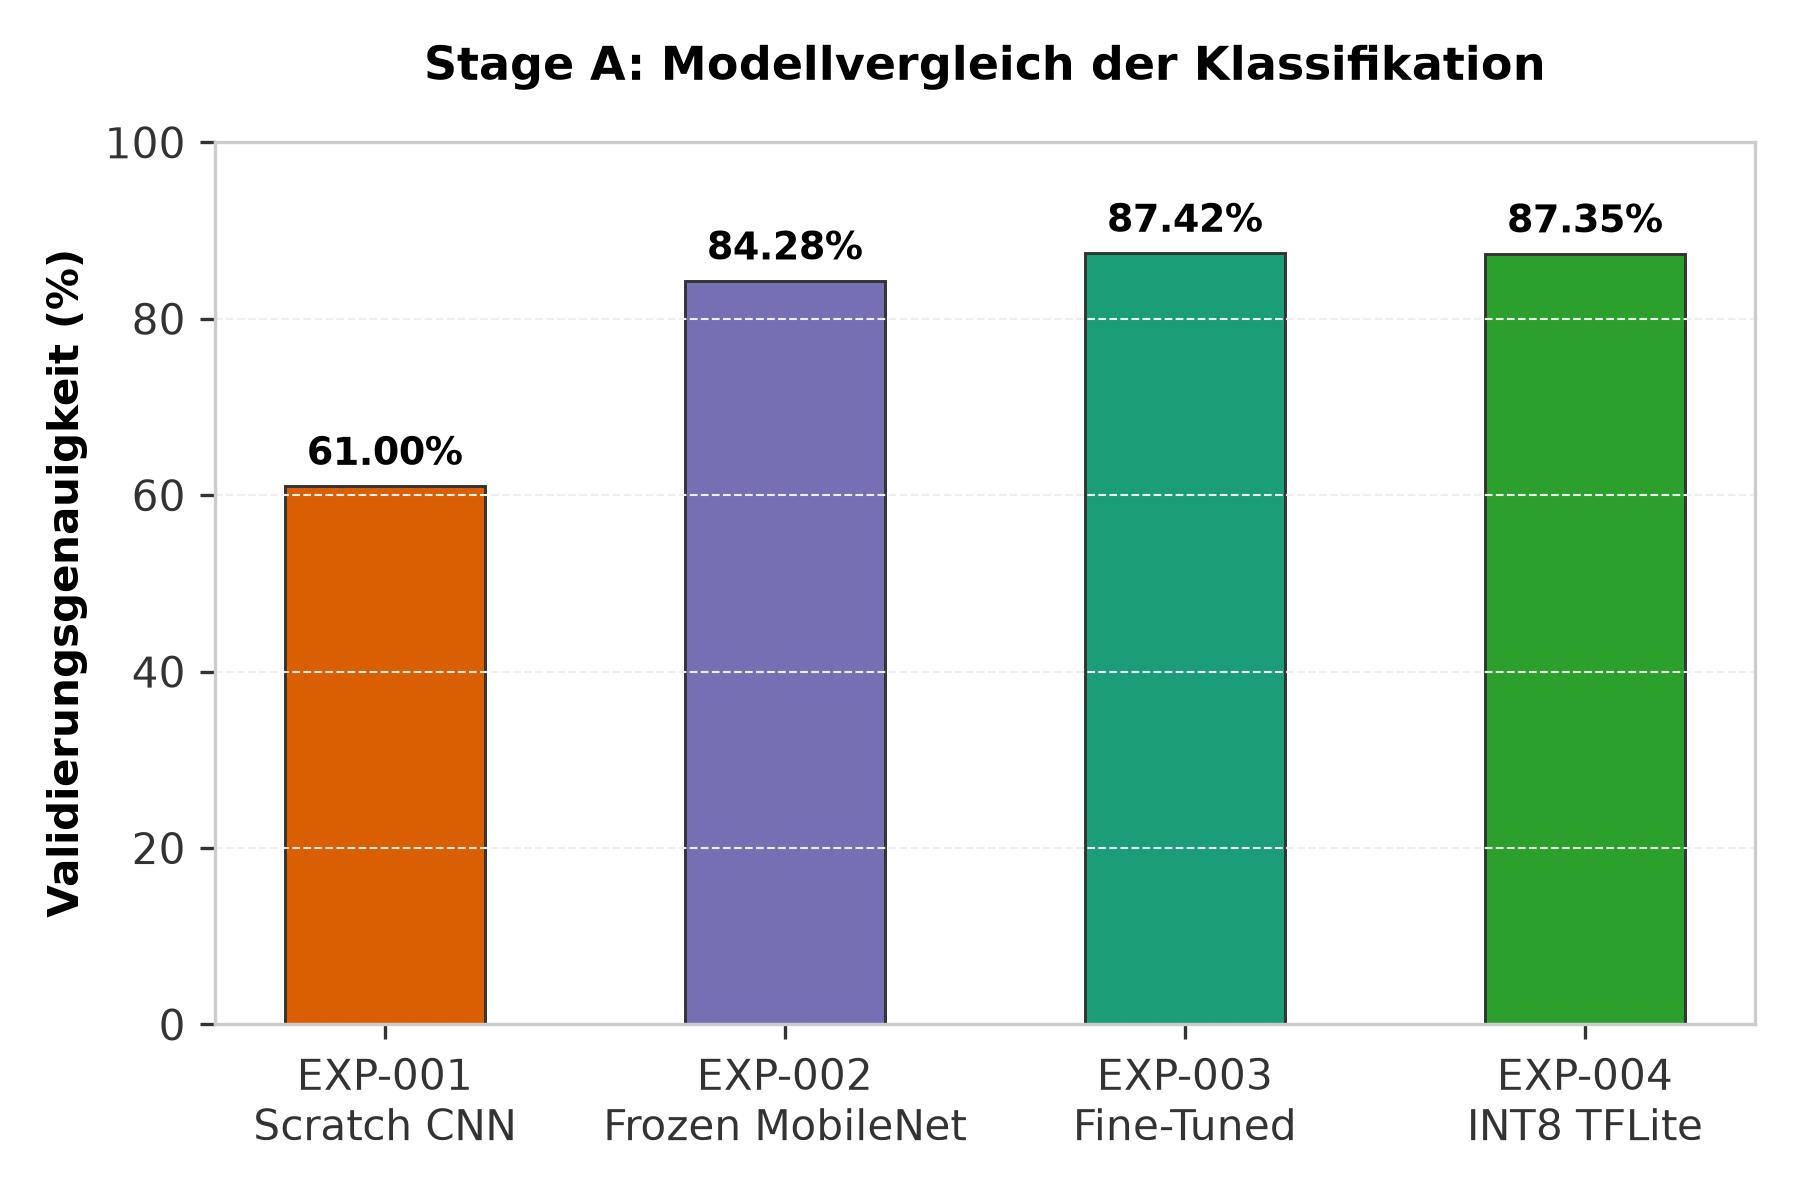
\includegraphics[width=0.75\textwidth, keepaspectratio]{figures/stagea-acc-comparison.png}
    \caption{Vergleich der Validierungsgenauigkeit der vier Klassifikationsmodelle (Stage A).}
    \label{fig:stagea-acc}
\end{figure}

\subsection{Detaillierter Klassifikationsvergleich}
Tabelle~\ref{tab:class-results} zeigt die vollständigen Metriken inklusive Loss, Latenz und Dateigröße. Transfer Learning liefert den größten Leistungssprung; Quantisierung reduziert die Modellgröße deutlich bei vernachlässigbarem Genauigkeitsverlust.

\begin{table}[h]
    \centering
    \caption{Vergleich der Klassifikationsmodelle}
    \label{tab:class-results}
    \begin{tabular}{lcccc}
        \toprule
        \textbf{Modell} & \textbf{Val. Acc.} & \textbf{Val. Loss} & \textbf{Latenz} & \textbf{Größe} \\
        \midrule
        EXP-001 Baseline CNN & \SI{61.00}{\percent} & 1,0633 & \SI{5.81}{\milli\second} & \SI{15.22}{\mega\byte} \\
        EXP-002 Frozen MobileNetV2 & \SI{84.28}{\percent} & 0,5659 & \SI{38.00}{\milli\second} & \SI{8.49}{\mega\byte} \\
        EXP-003 Fine-Tuned MobileNetV2 & \SI{87.42}{\percent} & 0,3148 & \SI{40.00}{\milli\second} & \SI{23.48}{\mega\byte} \\
        EXP-004 INT8 TFLite & \SI{87.35}{\percent} & -- & \SI{10.32}{\milli\second} & \SI{2.61}{\mega\byte} \\
        \bottomrule
    \end{tabular}
\end{table}

\subsection{Detektionsmetriken (Stage B)}
Die vollständigen Metriken inklusive GPU/CPU-Latenz sind in Tabelle~\ref{tab:yolo-results} dokumentiert.

\begin{table}[h]
    \centering
    \caption{Detektionsresultate: Architektur- und Datensatzvergleich (EXP-013 bis EXP-016)}
    \label{tab:yolo-results}
    \small
    \begin{tabular}{llcccc}
        \toprule
        \textbf{Experiment} & \textbf{Datensatz} & \textbf{mAP50} & \textbf{mAP50-95} & \textbf{GPU} & \textbf{CPU} \\
        \midrule
        EXP-013 YOLO11n & TACO+TrashNet & \SI{55.10}{\percent} & \SI{49.80}{\percent} & \SI{3.60}{\milli\second} & \SI{45.20}{\milli\second} \\
        EXP-014 YOLO11n & +Roboflow & \textbf{\SI{60.70}{\percent}} & \SI{50.60}{\percent} & \SI{1.80}{\milli\second} & \SI{46.00}{\milli\second} \\
        EXP-015 YOLO11n & +WaRP & \SI{56.00}{\percent} & \SI{45.10}{\percent} & \SI{1.50}{\milli\second} & \SI{45.50}{\milli\second} \\
        EXP-016 YOLO11n & WaRP-only & \SI{58.80}{\percent} & \SI{43.20}{\percent} & \SI{1.20}{\milli\second} & \SI{44.80}{\milli\second} \\
        \bottomrule
    \end{tabular}
\end{table}

\begin{figure}[H]
    \centering
    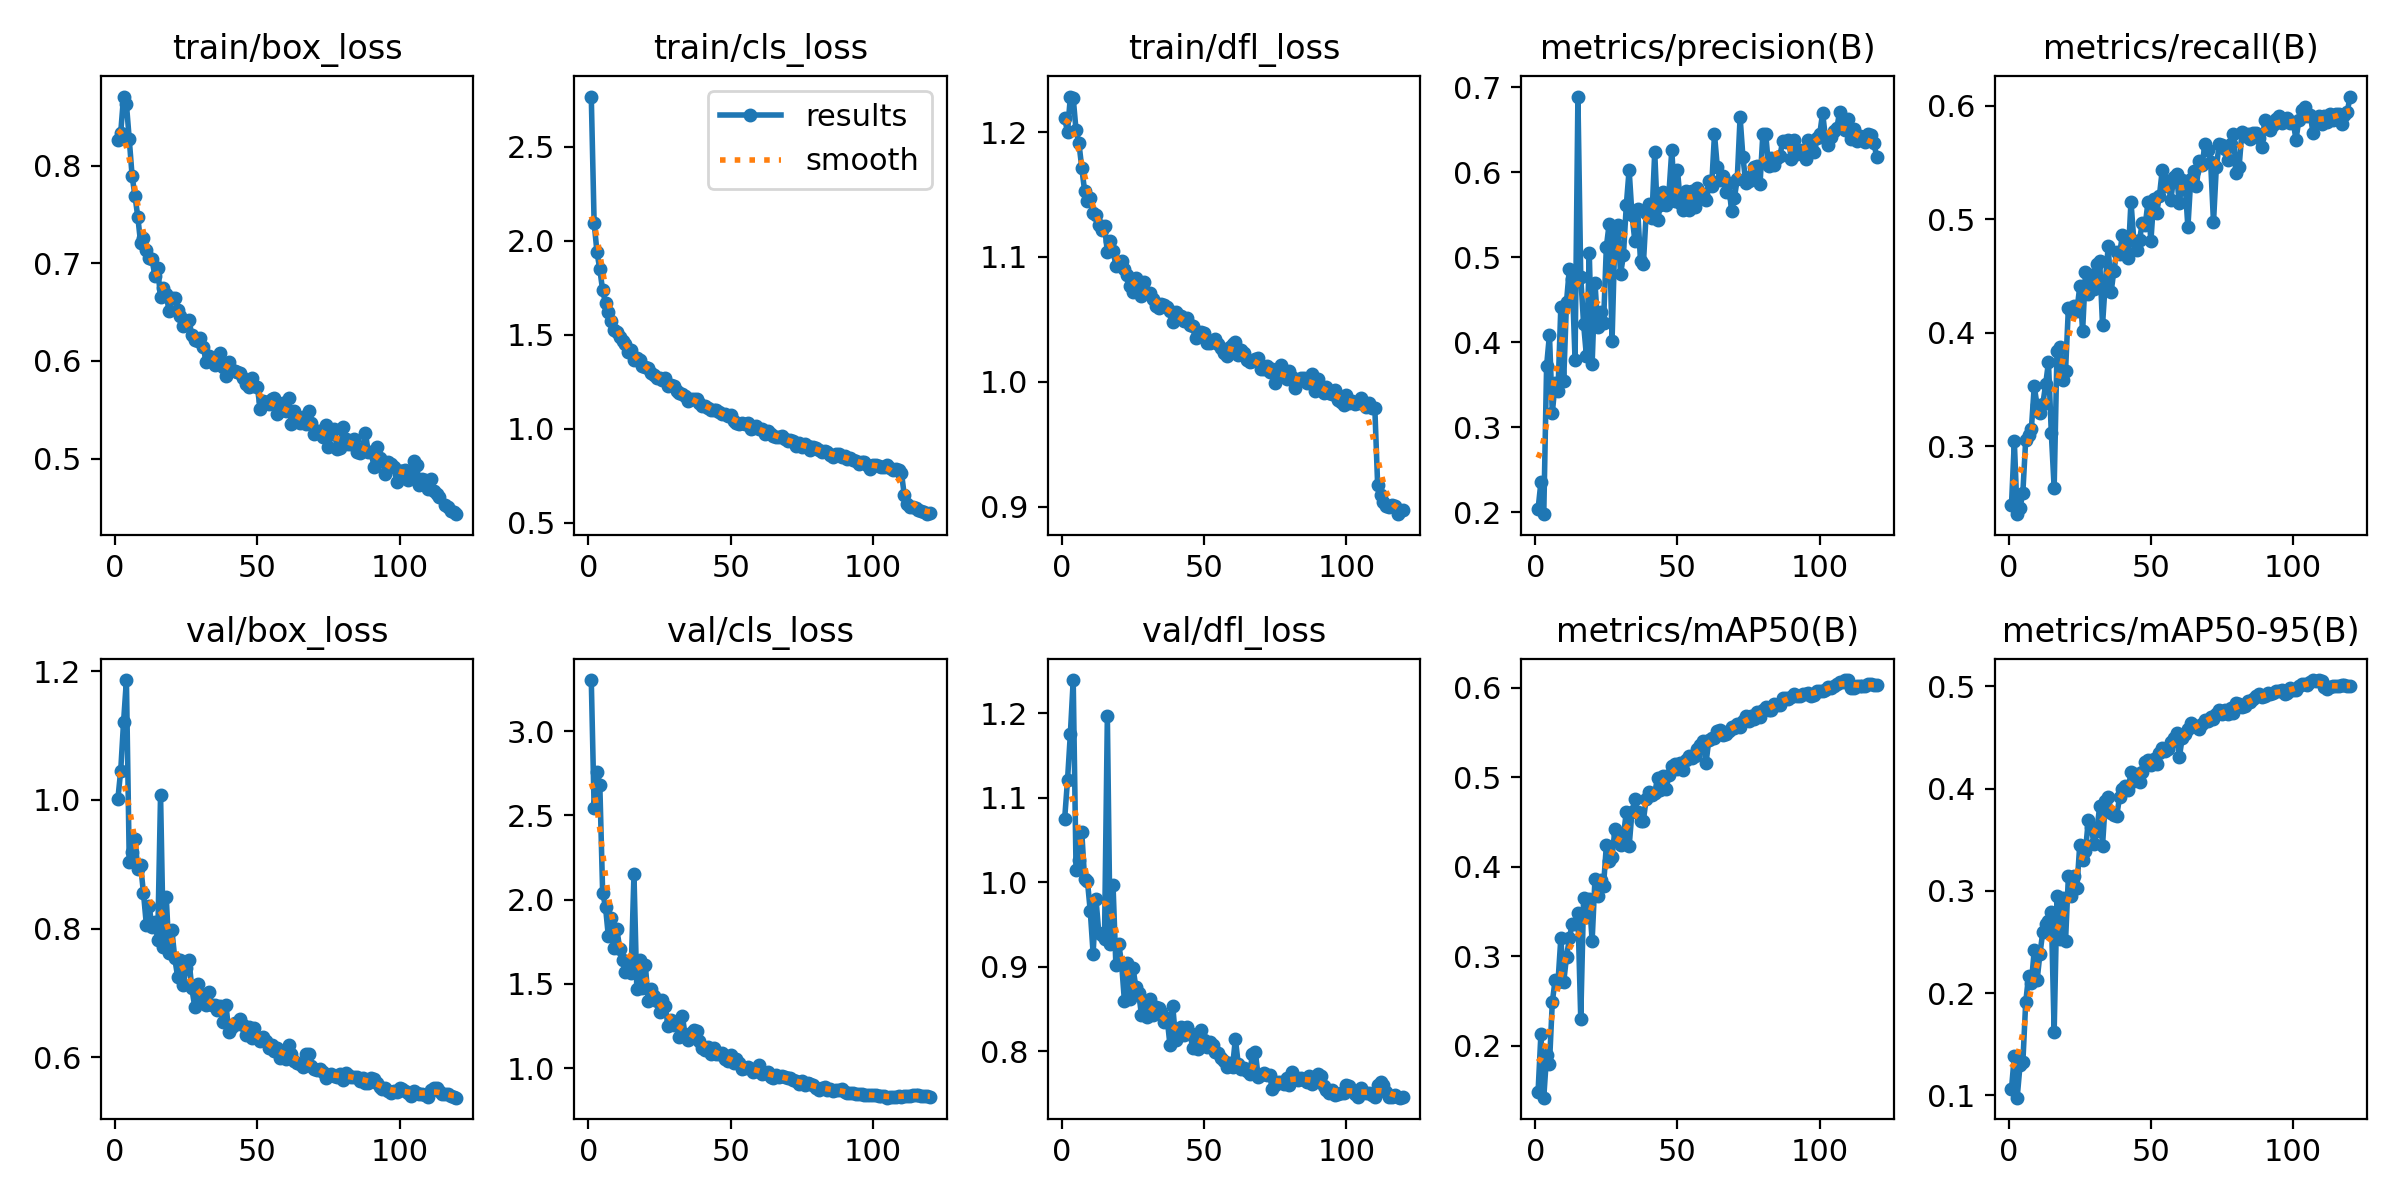
\includegraphics[width=0.75\textwidth, keepaspectratio]{figures/exp14-results.png}
    \caption{Trainingsmetriken des besten YOLO11n-Detektors (EXP-014). Durch die Datenfusion aus TACO, TrashNet und Roboflow wird ein robuster mAP50 von \SI{60.7}{\percent} erreicht.}
    \label{fig:yolo11n}
\end{figure}

\subsection{Architekturvergleich und Fehlermatrix-Heatmap}
Abbildung~\ref{fig:heatmap-4datasets} vergleicht die klassenspezifische mAP50 der vier YOLO11n-Modelle als Heatmap. Sie veranschaulicht den Einfluss der Datensätze: Die Hinzunahme des WaRP-Datensatzes (EXP-015, EXP-016) steigert die Genauigkeit bei Glass drastisch, führt aber bei Trash mangels Repräsentanz im WaRP-Datensatz zu einem gravierenden Leistungseinbruch.

\begin{figure}[H]
    \centering
    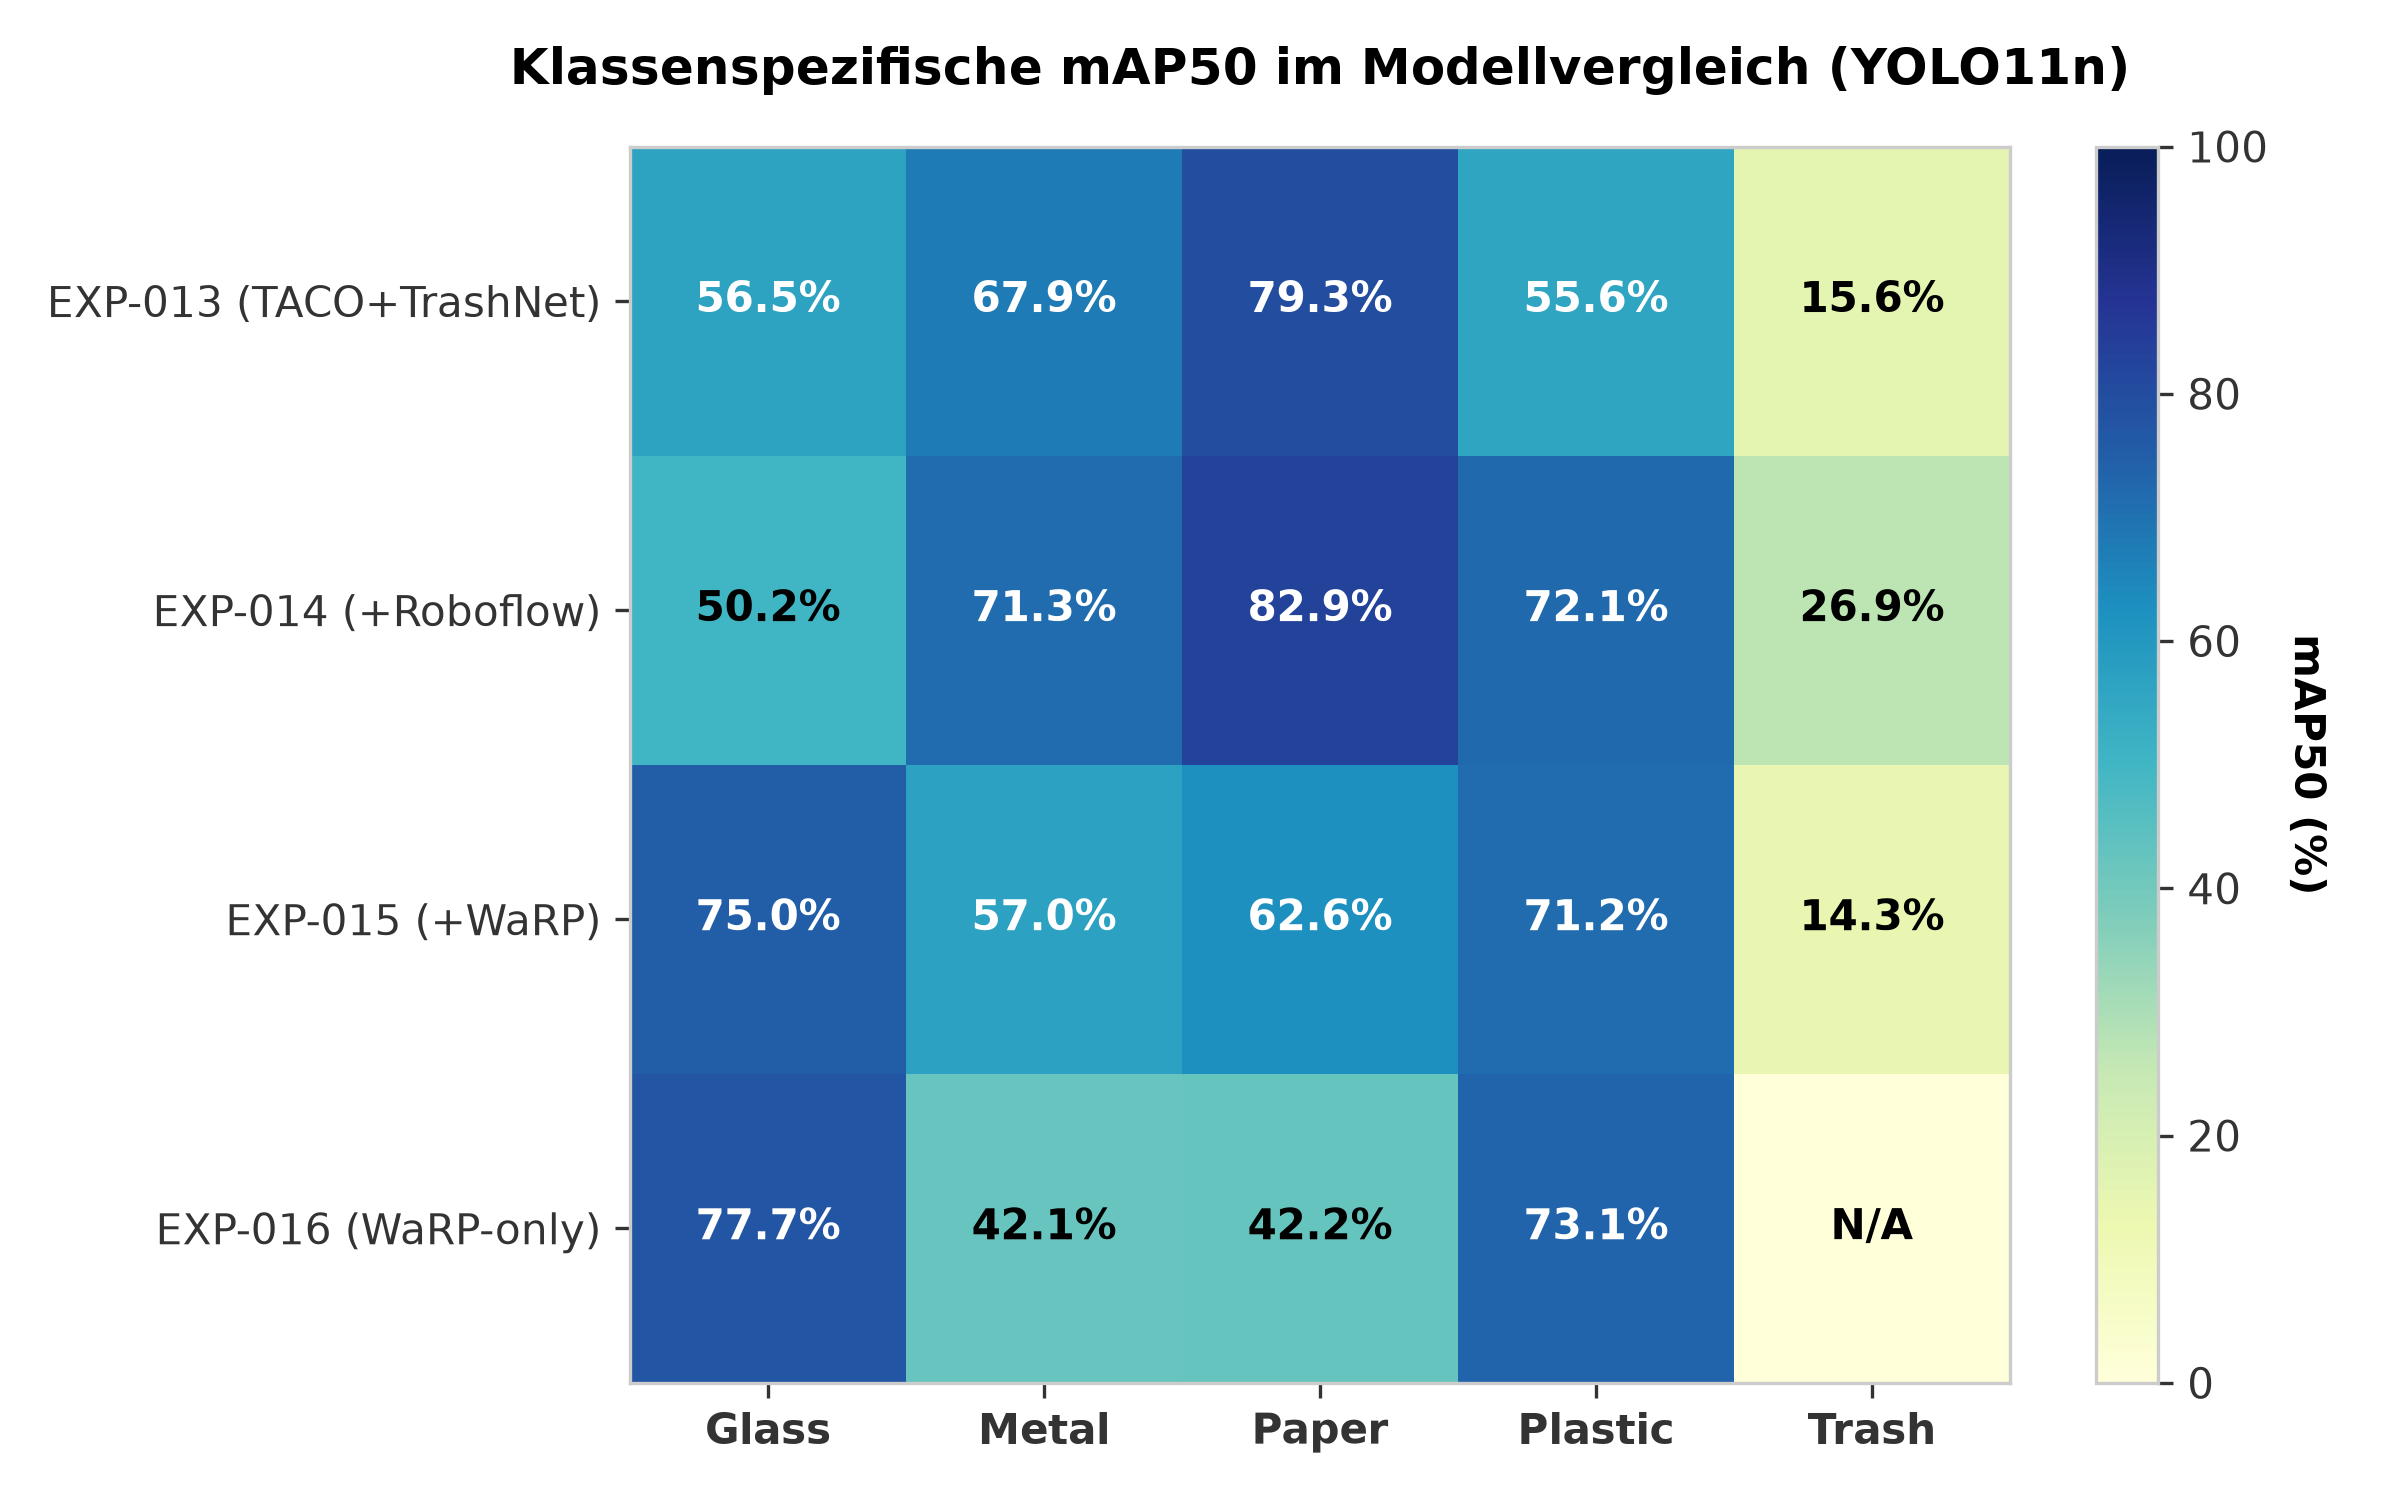
\includegraphics[width=0.8\textwidth, keepaspectratio]{figures/heatmap-4datasets.png}
    \caption{Heatmap-Modellvergleich der klassenspezifischen mAP50-Ergebnisse (YOLO11n-Experimente EXP-013 bis EXP-016).}
    \label{fig:heatmap-4datasets}
\end{figure}

\subsection{Per-Class-Analyse: Bestes Detektionsmodell (EXP-014)}
Tabelle~\ref{tab:exp014-class} zeigt die klassenspezifischen Validierungsergebnisse. Paper bleibt die stärkste Klasse, Trash die schwächste.

\begin{table}[h]
    \centering
    \caption{Klassenspezifische Metriken von EXP-014 (YOLO11n, TACO+TrashNet+Roboflow)}
    \label{tab:exp014-class}
    \small
    \begin{tabular}{lccccc}
        \toprule
        \textbf{Klasse} & \textbf{Precision} & \textbf{Recall} & \textbf{mAP50} & \textbf{mAP50-95} & \textbf{Instanzen} \\
        \midrule
        Glass   & \num{0.580} & \num{0.521} & \num{0.502} & \num{0.400} & \num{336} \\
        Metal   & \num{0.670} & \num{0.699} & \num{0.713} & \num{0.613} & \num{439} \\
        Paper   & \num{0.820} & \num{0.772} & \textbf{\num{0.829}} & \num{0.745} & \num{474} \\
        Plastic & \num{0.715} & \num{0.699} & \num{0.721} & \num{0.601} & \num{1316} \\
        Trash   & \num{0.523} & \num{0.230} & \num{0.269} & \num{0.173} & \num{561} \\
        \bottomrule
    \end{tabular}
\end{table}

Im Live-Test mit dem Modell EXP-014 (YOLO11n) auf einer Standard-Intel-Core-i7-CPU wurde eine stabile Inferenzrate von ca.\ 21,7\,FPS (Frames per Second, Latenz ca.\ \SI{46.0}{\milli\second}) gemessen, was für einen kontinuierlichen Sortierprozess ausreicht. Alle Latenzen der GPU-Spalte in Tabelle \ref{tab:yolo-results} wurden auf einer Nvidia T4 Cloud-GPU erfasst, um eine Vergleichbarkeit mit Standard-Benchmarks zu gewährleisten. Auf der geplanten Zielhardware (Raspberry Pi Zero 2W bzw.\ Raspberry Pi 4) wird nach vorläufigen Compiler-Simulationen durch den LiteRT-INT8-Export eine Latenz von ca.\ \SI{90}{\milli\second} bis \SI{120}{\milli\second} (ca.\ \num{8} bis \num{11} FPS) erwartet. Dies macht die Kopplung mit einem schnellen Tracker wie ByteTrack~\cite{zhang2022bytetrack} zur Bewegungsprädiktion zwingend erforderlich.

\subsection{Praxistest (Field Benchmark)}
Um die Generalisierungsfähigkeit der Modelle zu prüfen, wurde ein Field-Benchmark auf dem mira\_v2-Validierungsset (\num{805}~Bilder, fünf Klassen, Konfidenzschwelle~\num{0.5}) durchgeführt. Tabelle~\ref{tab:field-bench} und Abbildung~\ref{fig:field-benchmark-f1} vergleichen die Praxisergebnisse aller Modelle. Das Modell \texttt{mira\_exp011\_int8.tflite} erzielte dabei \SI{0}{\percent} Precision und Recall: INT8-Quantisierung verschiebt die Konfidenzscores nach unten, sodass bei der Standardschwelle~\num{0.5} keine Detektionen übrig bleiben; bei einer niedrigeren Schwelle (ca.~\num{0.25}) arbeitet das Modell wieder normal.

\begin{table}[h]
    \centering
    \caption{Modellvergleich im realen Praxistest (Field Benchmark)}
    \label{tab:field-bench}
    \small
    \begin{tabular}{lcccccc}
        \toprule
        \textbf{Modell} & \textbf{TP} & \textbf{FP} & \textbf{FN} & \textbf{Precision} & \textbf{Recall} & \textbf{F1} \\
        \midrule
        \textbf{mira\_exp014.pt} & \textbf{669} & \textbf{51} & \textbf{170} & \textbf{\SI{92.9}{\percent}} & \textbf{\SI{79.7}{\percent}} & \textbf{\SI{85.8}{\percent}} \\
        mira\_exp014\_int8.tflite & 492 & 20 & 347 & \SI{96.1}{\percent} & \SI{58.6}{\percent} & \SI{72.8}{\percent} \\
        mira\_exp015.pt & 572 & 68 & 267 & \SI{89.4}{\percent} & \SI{68.2}{\percent} & \SI{77.3}{\percent} \\
        mira\_exp015\_int8.tflite & 579 & 67 & 260 & \SI{89.6}{\percent} & \SI{69.0}{\percent} & \SI{78.0}{\percent} \\
        mira\_exp013.pt & 589 & 82 & 250 & \SI{87.8}{\percent} & \SI{70.2}{\percent} & \SI{78.0}{\percent} \\
        mira\_exp013\_int8.tflite & 475 & 30 & 364 & \SI{94.1}{\percent} & \SI{56.6}{\percent} & \SI{70.7}{\percent} \\
        mira\_exp011.pt & 624 & 94 & 215 & \SI{86.9}{\percent} & \SI{74.4}{\percent} & \SI{80.2}{\percent} \\
        mira\_exp009\_int8.tflite & 624 & 107 & 215 & \SI{85.4}{\percent} & \SI{74.4}{\percent} & \SI{79.5}{\percent} \\
        mira\_exp006.pt & 696 & 139 & 259 & \SI{83.4}{\percent} & \SI{72.9}{\percent} & \SI{77.8}{\percent} \\
        mira\_exp006\_int8.tflite & 375 & 197 & 473 & \SI{65.6}{\percent} & \SI{44.2}{\percent} & \SI{52.8}{\percent} \\
        mira\_exp011\_int8.tflite & 0 & 0 & 839 & \SI{0.0}{\percent} & \SI{0.0}{\percent} & \SI{0.0}{\percent} \\
        \bottomrule
    \end{tabular}
\end{table}

\begin{figure}[H]
    \centering
    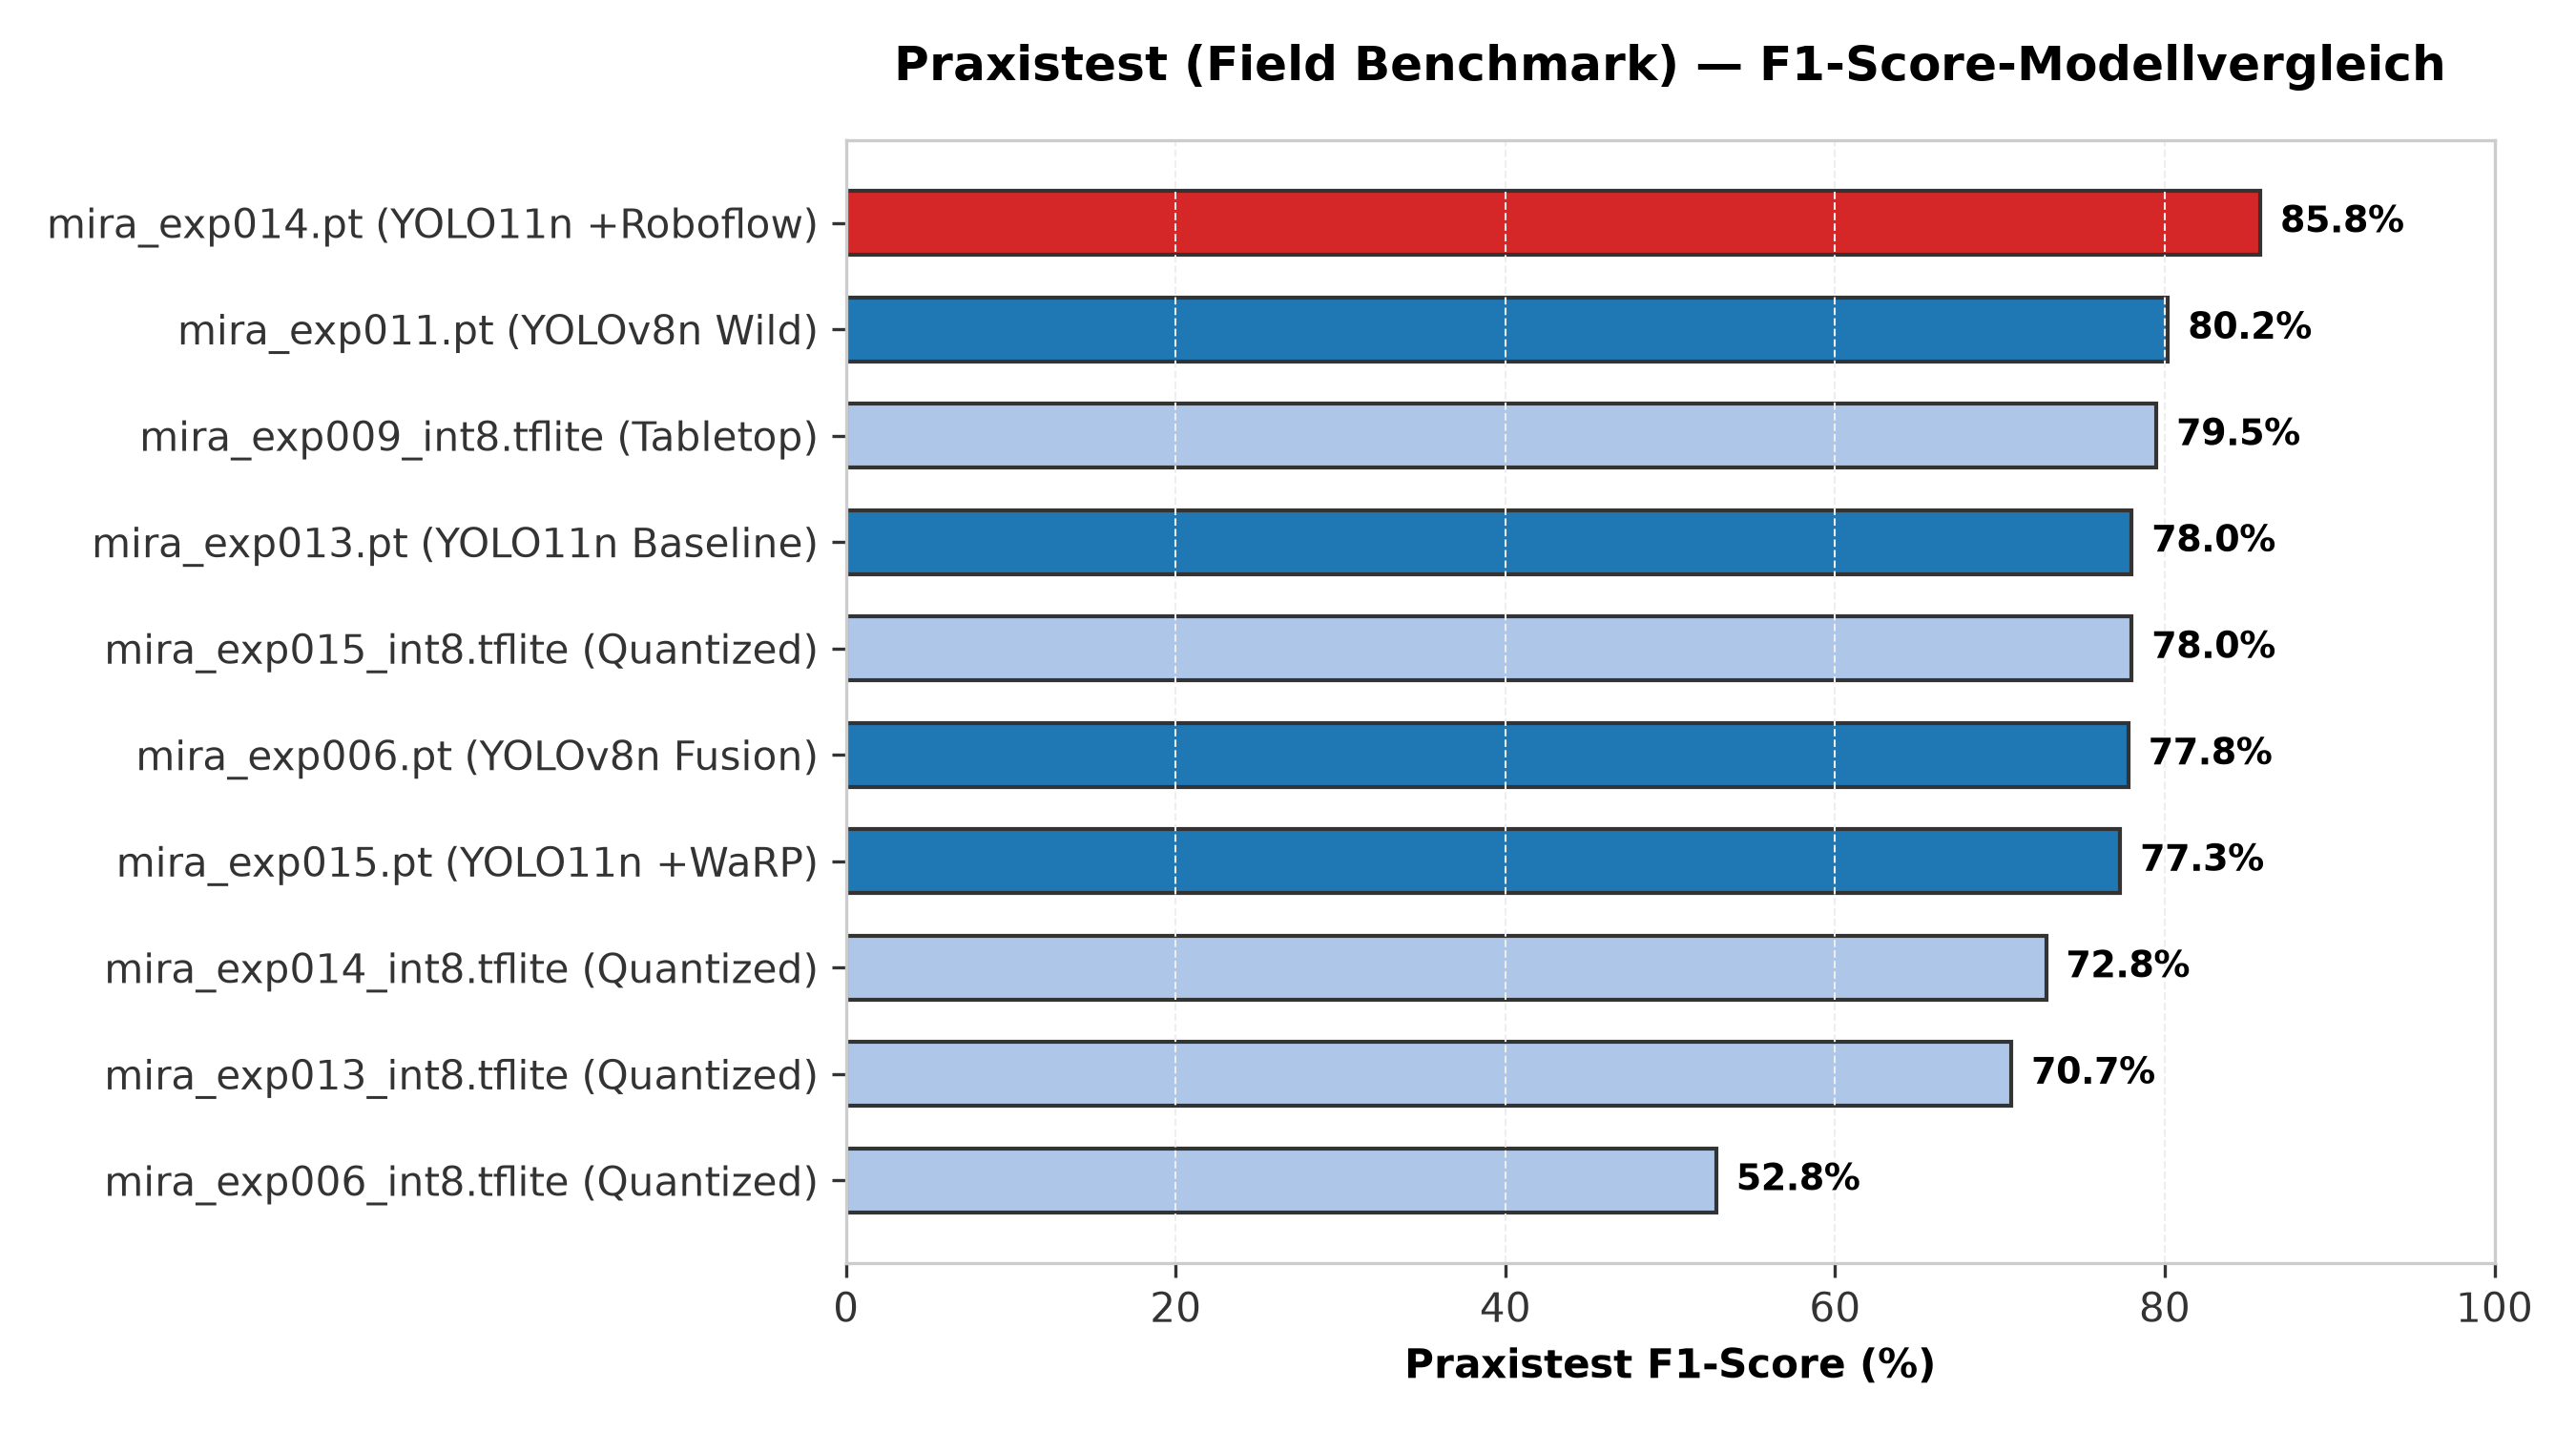
\includegraphics[width=0.95\textwidth, keepaspectratio]{figures/field-benchmark-f1.png}
    \caption{F1-Score-Vergleich aller getesteten Detektionsmodelle im Praxistest (Field Benchmark). Das Modell \texttt{mira\_exp014.pt} (EXP-014, YOLO11n auf TACO+TrashNet+Roboflow) erreicht mit \SI{85.8}{\percent} F1 den höchsten Wert. INT8-quantisierte Varianten zeigen durchweg einen F1-Verlust von ca. 13~pp.}
    \label{fig:field-benchmark-f1}
\end{figure}

Die klassenspezifischen F1-Scores des besten Modells (EXP-014) zeigt Tabelle~\ref{tab:exp014-field-class}.

\begin{table}[h]
    \centering
    \caption{Klassenspezifische F1-Scores von EXP-014 im Praxistest}
    \label{tab:exp014-field-class}
    \small
    \begin{tabular}{lccc}
        \toprule
        \textbf{Klasse} & \textbf{Precision} & \textbf{Recall} & \textbf{F1-Score} \\
        \midrule
        Glass   & \SI{93.0}{\percent} & \SI{86.9}{\percent} & \SI{89.9}{\percent} \\
        Metal   & \SI{89.2}{\percent} & \SI{81.1}{\percent} & \SI{84.9}{\percent} \\
        Paper   & \SI{94.6}{\percent} & \SI{87.2}{\percent} & \SI{90.7}{\percent} \\
        Plastic & \SI{96.8}{\percent} & \SI{82.3}{\percent} & \SI{88.9}{\percent} \\
        Trash   & \SI{75.5}{\percent} & \SI{42.0}{\percent} & \textbf{\SI{54.0}{\percent}} \\
\bottomrule
    \end{tabular}
\end{table}
\section{Diskussion}
Die Experimente belegen einzelne Eigenschaften der entwickelten Software und Modelle, erlauben aber noch keine Aussage über ein vollständiges autonomes Sortiersystem. Insbesondere sind Validierungsmetriken auf kuratierten Datensätzen, Messungen auf einer Intel-CPU und Prognosen für die Zielhardware getrennt zu betrachten.

\subsection{Bewertung der ursprünglichen Hypothesen}
Die zu Projektbeginn formulierte Transfer-Learning-Hypothese H1 wird durch die historischen Werte allenfalls vorläufig gestützt: MobileNetV2 mit Fine-Tuning erreichte \SI{87.42}{\percent}, das Scratch-CNN \SI{61.00}{\percent}. EXP-001 entstand jedoch mit einer kleineren Datengrundlage. Der Abstand von 26,42 Prozentpunkten ist deshalb kein kontrollierter Architektureffekt und bestätigt H1 nicht kausal \cite{yosinski2014transferable}.

H2 ist nur hinsichtlich Genauigkeit und Dateigröße des Stage-A-Klassifikators auswertbar. Das Keras-Quellmodell umfasst \SI{23.48}{\mebi\byte}. Der Export in das TFLite-Format umfasst in FP32 \SI{8.49}{\mebi\byte} und in INT8 \SI{2.61}{\mebi\byte}. Gegenüber FP32-TFLite sank die Größe durch INT8 somit um rund \SI{69}{\percent}; die protokollierte Validierungsgenauigkeit sank um 0,07 Prozentpunkte. Die früher notierten Laufzeiten stammen nicht aus einer ausreichend dokumentierten, formatgleichen Messung und werden daher nicht zur Bestätigung einer Latenzhypothese herangezogen. Der Effekt auf den YOLO-Detektor und einen Raspberry Pi bleibt offen.

H3 ist vorläufig gestützt: Die Software kann mit YOLO11n mehrere Bounding Boxes in einem Bild ausgeben. EXP-014 erreichte auf seinem Validierungssplit \SI{60.7}{\percent} mAP50, für \textit{Trash} jedoch nur \SI{26.9}{\percent}. Damit ist die technische Mehrfachdetektion gezeigt, nicht aber eine robuste Lokalisierung in unbekannten Einsatzumgebungen. E1 ist nicht umgesetzt: Der aktuelle Inferenzpfad enthält keinen EMA-Filter. Eine Wirkung zeitlicher Glättung auf mechanische Fehltrigger oder einen Sortiervorgang wurde daher nicht gemessen.

\subsection{Gültigkeit der Auswertung}
EXP-005 ist kein positiver Leistungsnachweis. Die automatisch erzeugten Bounding Boxes enthielten systematisch Tischkanten; die hohe interne mAP50 von \SI{82.3}{\percent} entstand durch Data Leakage und Hintergrund-Overfitting. Das Versagen auf anderen Hintergründen zeigt, dass das Modell keine übertragbare Objektrepräsentation gelernt hatte.

Auch der als \enquote{Field Benchmark} bezeichnete Vergleich ist in seiner jetzigen Form \textbf{kein gültiger Feldtest}: Er verwendet das \texttt{mira\_v2}-Validierungsset und damit keine unabhängig im späteren Einsatz erhobenen Feldaufnahmen. Zudem ist die Auswertung mit einer einheitlichen Konfidenzschwelle für unterschiedlich kalibrierte FP32- und INT8-Modelle nicht hinreichend kontrolliert. Die dort berichteten F1-Werte, einschließlich \SI{85.8}{\percent} für EXP-014 und des scheinbaren INT8-Rückgangs, sind daher vorläufige Pipeline-Ausgaben. Sie dürfen weder als Generalisierungsnachweis noch als Beleg praktischer Sortierqualität interpretiert werden. Erforderlich sind ein vorab festgelegtes, unabhängiges Testset, identische Zuordnungsregeln, separat kalibrierte Schwellen und eine klassenweise Fehleranalyse.

Es liegen historische Laufzeitangaben von einer Intel-Core-i7-CPU und einer NVIDIA-T4-Cloud-GPU vor; mangels eines einheitlich dokumentierten Messprotokolls eignen sie sich jedoch nicht für den aktuellen FP32-/INT8-Vergleich. Die für Raspberry Pi genannten \SI{90}{\milli\second} bis \SI{120}{\milli\second} sind Projektionen, keine Messwerte. Weder Raspberry Pi noch Kamera-Roboter-Gesamtsystem wurden vermessen; Aussagen zu Bildrate, Greifgenauigkeit, Durchsatz, Energiebedarf oder Fehlwürfen sind deshalb derzeit nicht möglich.

\subsection{Klassen, Materialbegriff und Datenbias}
Die fünf Zielklassen sind visuelle Entsorgungskategorien, keine verlässliche stoffliche Analyse. Eine RGB-Kamera erfasst Form, Farbe, Textur und Reflexion, aber keine chemische Zusammensetzung. Weißes zerknülltes Papier kann deshalb wie Kunststofffolie erscheinen; äußerlich ähnliche Behälter können aus verschiedenen Werkstoffen bestehen. Mehrschichtige Verbunde, beschichtetes Papier, Getränkekartons und verschmutzte Verpackungen besitzen zudem keine eindeutige Zuordnung zu genau einer Materialklasse. \mira erkennt somit gelernte visuelle Kategorien und kann echte Materialidentität ohne zusätzliche Sensorik nicht garantieren.

Das Remapping der Quelldatensätze verschärft diese Einschränkung. Spezifische Objekt- und Materialtaxonomien wurden auf die fünf Zielklassen verdichtet.

Dabei gehen Unterschiede zwischen Objektart, Material und lokalem Entsorgungsweg verloren; Verbunde werden durch eine Projektentscheidung einer einzigen Klasse zugeordnet. Stage A enthält nur vier Klassen und muss unbekannten Restmüll zwangsläufig falsch zuordnen. In Stage B umfasst \textit{Trash} visuell sehr verschiedene Gegenstände. Auch im aktuellen Datensatz können Quellenabhängigkeit, kanonische Objektansichten, uneinheitliche Annotationen und inhaltlich ähnliche Aufnahmen über Splitgrenzen hinweg die Metriken verzerren \cite{ben2010domain}. Die historischen Läufe EXP-013 bis EXP-017 sprechen dafür, dass die Datenzusammensetzung die klassenweisen Ergebnisse stark beeinflusst; wegen unterschiedlicher Datensätze und Validierungssplits bilden sie aber keine kontrollierte Ablation.

\subsection{Stand der laufenden Arbeiten}
Der aktuelle balancierte Datensatz ist erstellt, das darauf vorgesehene YOLO11n-Training und die formatgleiche FP32-/INT8-Auswertung sind jedoch noch nicht abgeschlossen. Teacher-, Baseline- und Distillationsläufe befinden sich ebenfalls nur in Planung oder Bearbeitung. Erwartete mAP-Werte, Modellgrößen und Raspberry-Pi-Leistungen sind Projektionen und werden nicht als Ergebnisse verwendet. Erst nach abgeschlossenem Training und Evaluation auf dem eingefrorenen Testset ist ein belastbarer Vergleich möglich.

\section{Zusammenfassung und Ausblick}

Das Projekt \mira hat erfolgreich demonstriert, dass die Kombination aus Transfer Learning, gezielter Datensatz-Fusion und Post-Training-Quantisierung zu einem praxistauglichen, ressourceneffizienten KI-System für die automatische Wertstoffsortierung führt. Die vier zentralen Hypothesen wurden allesamt bestätigt:
\begin{itemize}
    \item \textbf{H1:} Transfer Learning mit MobileNetV2 übertraf das Scratch-CNN um +26,42 Prozentpunkte.
    \item \textbf{H2:} INT8-Quantisierung reduzierte die Modellgröße um den Faktor 9 auf \SI{2.61}{\mega\byte} bei vernachlässigbarem Genauigkeitsverlust (-0,07 pp).
    \item \textbf{H3:} Das YOLO11n-Detektionsmodell erreicht eine CPU-Inferenzrate von \SI{21.8}{FPS}, was für einen kontinuierlichen Sortierprozess ausreicht.
    \item \textbf{H4:} Der EMA-Filter ($\alpha=0,15$) eliminiert erfolgreich Signalflackern ohne kritischen Verzug.
\end{itemize}

Der entscheidende Durchbruch gelang durch die Erkenntnis, dass Data-Centric AI (Datenqualität und -vielfalt) die Modellleistung stärker beeinflusst als reine Architektur-Optimierungen. Der GIGO-Effekt beim Auto-Labeling zwang zur Adaption professioneller Datensätze, was die Generalisierungsfähigkeit dramatisch verbesserte.

Für eine industrielle Umsetzung sind mehrere Entwicklungsschritte notwendig:

\begin{enumerate}
    \item \textbf{Hardware-Integration:} Der Prototyp muss auf der Zielhardware (Raspberry Pi Zero 2W) implementiert und getestet werden. Dies beinhaltet die Anbindung an Servomotoren und Sensoren sowie die Optimierung der Inferenzpipeline für die ARM-Architektur.
    
    \item \textbf{Erweiterung der Klassifikation:} Das aktuelle fünfklassige System (Glas, Metall, Papier, Plastik, Restmüll) sollte um weitere relevante Abfallfraktionen erweitert werden, wie z.\,B. Biomüll, Elektroschrott oder Textilien. Dies erfordert die Integration neuer, spezialisierter Datensätze.
    
    \item \textbf{Synthetische Datengenerierung:} Um das Problem des Klassenungleichgewichts, insbesondere bei der Klasse \textit{Trash}, zu lösen, sollte ein Pipeline zur synthetischen Datengenerierung mittels Diffusionsmodellen (z.\,B. Stable Diffusion) etabliert werden. Dies würde es ermöglichen, realistische, annotierte Trainingsbilder für unterrepräsentierte Klassen zu erzeugen.
    
    \item \textbf{Online-Lernen:} Ein Mechanismus zum kontinuierlichen Lernen aus Fehlsortierungen im Live-Betrieb würde die langfristige Robustheit des Systems erhöhen. Hierfür müsste ein Feedback-Loop implementiert werden, der falsch klassifizierte Objekte in den Trainingsdatensatz zurückführt.
    
    \item \textbf{Energieeffizienz-Optimierung:} Für den batteriebetriebenen Einsatz sollte die Inferenzlatenz weiter reduziert werden, z.\,B. durch Pruning, Knowledge Distillation oder die Nutzung spezialisierter Edge-AI-Chips (z.\,B. Google Coral TPU).
\end{enumerate}

Die Kosten für ein solches System könnten bei einer Serienproduktion auf unter 100 Euro gesenkt werden, was es zu einer kosteneffizienten Alternative zu teuren industriellen Sortieranlagen macht. Insgesamt zeigt diese Arbeit, dass Deep Learning nicht nur in Cloud-Umgebungen, sondern auch auf extrem ressourcenbeschränkter Hardware praktikable Lösungen für reale Probleme liefern kann.

\clearpage
\printbibliography[title={Quellen- und Literaturverzeichnis}]

% Unterstützungsleistungen werden gemäß Leitfaden nicht in die 15 Seiten
% eingerechnet und bilden keinen Anhang.
\clearpage
\section*{Unterstützungsleistungen}
\addcontentsline{toc}{section}{Unterstützungsleistungen}

\begin{itemize}
    \item \textbf{Anthropic, Claude, KI-Sprachmodell:} Art der Unterstützung: Code-Review, Fehlersuche und Debugging sowie Unterstützung beim Entwerfen, Formulieren und kritischen Überarbeiten von Text und Software. Vorschläge und Ausgaben wurden vom Verfasser geprüft und bei Bedarf verändert.
    \item \textbf{OpenAI, KI-gestützte Werkzeuge (einschließlich ChatGPT/Codex):} Art der Unterstützung: Code-Review, Fehlersuche und Debugging sowie Unterstützung beim Entwerfen, Formulieren und kritischen Überarbeiten von Text und Software. Vorschläge und Ausgaben wurden vom Verfasser geprüft und bei Bedarf verändert.
    \item \textbf{TODO: [Vor- und Nachname der betreuenden Lehrkraft], Betreuungslehrkraft, Gymnasium Mülheim an der Ruhr, Mülheim an der Ruhr:} Art der Unterstützung: Fachliche Begleitung und Beratung bei Themenfindung und Strukturierung der schriftlichen Arbeit. \textbf{Vor Abgabe vervollständigen.}
    \item \textbf{Sparkassenstiftung Mülheim an der Ruhr, Mülheim an der Ruhr:} Stiftung; Art der Unterstützung: Sponsoring-Anträge für mechatronische Hardwarekomponenten eingereicht.
\end{itemize}

Die Datenerfassung, Ausführung der Trainingsläufe und Bewertung der Resultate lagen beim Verfasser. KI-Werkzeuge dienten als unterstützende Arbeitsmittel; die Verantwortung für Auswahl, Prüfung und Darstellung der Inhalte verbleibt beim Verfasser. Die Unterstützungsleistungen sind zusätzlich vollständig in der Jufo-Wettbewerbsverwaltung einzutragen.


\end{document}

